\newpage
\newcommand{\CandidateChain}{\texttt{\color{AlgProcedureColor}candidate\textunderscore{}chain} }
\section{Task2}
During the second task,  the topics extracted in \textbf{Task 1}  are tracked throughout the years and fused together. The set of years to be merged  is indicated by the sequence $\mathcal Y = \{y_i\}_{i=0..18}$.
Two approaches were tested for solving this task:
\begin{itemize}
\item In the first method, topics between adjacent years are linked together, creating then a \textit{direct acyclic graph} of the topics. From this graph are extracted $K=20$ paths, representing the topic evolution. These are then merged in order to represent the final fused topics.
\item The second approach makes use of more information, and uses the similarity of each pair of topics between all the years in $\mathcal Y$. Using this similarity (after being appropriately weighted) chains of topics are computed using a greedy approach. Similarly to the previous approach, these chains are then merged together in order to create the fused topics.
\end{itemize}

\subsection{Keyword Similarity}\label{sec:keyword_similarity}
In order to determine if two topics are related, a metric describing the similarity between two keywords is necessary. This may be useful when trying assess the similarity between topics, especially if said topics do not share a great number of words, but have a lot of similar words in common. The keyword similarities considered for the project are two:
\begin{description}
	\item[Exact Match:] this is a rather simple similarity function, mapping to 1 only pairs of keywords represented by the same exact character sequence. This is a very conservative metric, with high precision but low recall.
	$$
	\KeywordScore(w_1,w_2) = \begin{cases}
	1 & \text{if $w_1 = w_2$}\\
	0 & \text{otherwise}
	\end{cases}
	$$
	\item[Jaccard Similarity:] the similarity between two keywords  is computed  using their \textit{bag-of-words} representation; each keyword is seen as a sequence of smaller words (using white-spaces as delimiter), which are then compared utilizing the \textit{Jaccard Similarity}.\\
	For example consider the keywords: \textbf{\enquote{brown fox}}, and \textbf{\enquote{quick fox}}, the estimated similarity score is given by 
	$$
	\KeywordScore(\textbf{\enquote{brown fox}}, \textbf{\enquote{quick fox}})  = %
	\frac{|\{\textbf{\enquote{fox}}\}|}{|\{\textbf{\enquote{brown}}, \textbf{\enquote{quick}}, \textbf{\enquote{fox}}\}|}= \frac{1}{3}
	$$
	This similarity suffers the opposite problem, since it may give an higher similarity value then it  should, particularly if frequent words are in both keywords.
\end{description}
\subsection{Topic-Pairs Score}\label{sec:topic_score}
The keyword similarity information described in the previous section is then utilized in order to associate topics from different years. This is performed using a score function, and later on using said score to create a relation between nodes in different years. 
% TODO add a simple matrix as example
During the project development, several score-functions were tested, the main one were:
\begin{description}
	\item[Jaccard Similarity:] the jaccard similarity was also used for topics scoring, using the keyword sets associated to each topic. The jaccard score seems to be a simple but effective score, however, it suffers one major drawback: it is not possible to exploit the jaccard keyword similarity previously described in \cref{sec:keyword_similarity}. %and it requires topic to be a crisp set, and does not generalize to fuzzy ones (however, this is less problematic since crisp topics were mostly used in the project).
	$$\TopicScore(T_i,T_j) = \frac{|T_i\cap T_j|}{|T_i \cup T_j|}$$
	\item[Fuzzy Similarity] this similarity was an attempt at a generalization of the  jaccard similarity, while adapting fuzzy topics and exploiting the keyword similarities described before.
	Let $\Fuzzy{T_1}$ and $\Fuzzy{T_2}$ be two fuzzy topics (with respective membership functions $\mu_{\Fuzzy{T_i}}$ and $\mu_{\Fuzzy{T_j}}$)
	\begin{gather*}
		\mathbb I(\Fuzzy T_i,\Fuzzy T_j) = \Membership{\Fuzzy{T_i}}(w_1)\cdot \Membership{\Fuzzy{T_j}}(w_2)\cdot \KeywordScore(w_1,w_2)\\
		\mathbb U(\Fuzzy T_i,\Fuzzy T_j) = \sum_{w_1,w_2}\Membership{\Fuzzy{T_i}}(w_1)\cdot \KeywordScore(w_1,w_2) +  \sum_{w_1,w_2}\Membership{\Fuzzy{T_j}}(w_2)\cdot \KeywordScore(w_1,w_2) - \mathbb I(\Fuzzy T_i,\Fuzzy T_j)
	\end{gather*}
	$$
	\TopicScore(\Fuzzy{T_i}, \Fuzzy{T_j}) = \frac{\displaystyle\phantom{\bigg(}\mathbb I(\Fuzzy T_i,\Fuzzy T_j)}{\displaystyle \phantom{\bigg(} \mathbb U(\Fuzzy T_i,\Fuzzy T_j)}
	$$
	This approach however yielded poor results, hence was quickly discarded.
	\item[Chamfer Similarity:] this similarity function is inspired by the \textit{chamfer distance} described in \cite{chamfer}. The score of a topic pair is given by the average keyword similarity of each node in the topic when mapped to the most similar word in the opposing topic. The averages from both topics are then summed, and the resulting value is the final score.
	$$
	\TopicScore(T_i,T_j) = \frac{1}{|T_i|}\sum_{w_{1}\in T_i}\max_{w_2\in T_j}\KeywordScore(w_1,w_2) + \frac{1}{|T_j|}\sum_{w_2\in T_j}\max_{w_1\in T_i} \KeywordScore(w_1,w_2)
	$$
	A problem  with this score function is that it tends to favor smaller topics (especially with one or two nodes), since their score usually vary more than bigger sized topics. This could be addressed by using the square root of the topic cardinality instead of the cardinality itself (however, this approach was not tested).
\end{description}



\subsection{Time-Fused Topics (First Attempt)}\label{sec:first_attempt}
In this section is described the first attempt at creating time-fused topics. Unfortunately, the results yielded poor accuracy and were heavily unbalanced, creating few topics with a great number of keywords. Nevertheless, the approach used is worth mentioning.

\paragraph{\textbf{Topic direct acyclic graph.}}
Using one of the previously described topic-pairs score functions, a \textit{Direct Acyclic Graph} (DAG) of topics was created. This graph encoded information about topic evolution throughout the years; it did so by containing several levels of nodes, where each level contained all the topics of a given year, see \cref{ifg:dag} for a better understanding.\\
More formally, let $G_{\DAG}$ be the topic DAG, then the nodes of this graph are the topics extracted\footnote{From the year 2000 to 2018 (included).} in the previous task; if $\mathcal{T}_y$ is the set containing all the topics estimated for year $y$, then the set of vertices $\Vertices_{\DAG}$ of $G_{\DAG}$ is defined as
$$
\Vertices_{\DAG} = \bigcup_{k=0}^{18} \mathcal{T}_{y_k}
$$
on the other hand, the set of edges is computed using the function $\TopicScore$; specifically, for a given year $y_{k}$, an edge $(T_i,T_j)\in \mathcal T_{y_k}\times\mathcal T_{y_{k+1}}$ is added to $G_{\DAG}$ if:
\begin{itemize}
	\item $T_j$ is the topic in $T_{y_{k+1}}$ that maximizes $\TopicScore(T_i,T_j)$,
	\item or $T_i$ is the topic in $T_{y_{k}}$ that maximizes $\TopicScore(T_i,T_j)$.
\end{itemize}
Hence the set of edges in $G_{\DAG}$ (denoted as $\Edges_{\DAG}$) is given by:
$$
\Edges_{\DAG} = \bigcup_{k=0}^{18-1} \Big(\overleftarrow{\Edges}_{y_k} \cup \overrightarrow{\Edges}_{y_k}\Big)
$$
with the sets $\overleftarrow{\Edges}_{y}$ and $\overrightarrow{\Edges}_{y}$ defined in the following manner:
\[
\overleftarrow{\Edges}_{y_k} = \Big\{(T_i, T_j) \in\mathcal T_{y_k}\times\mathcal T_{y_{k+1}}: T_j = \mathop{\mathrm{argmax}}_{\dot T\in \mathcal T_{y_{k+1}}} \{\TopicScore(T_i, \dot T)\}  \Big\}
\]
\[
\overrightarrow{\Edges}_{y_k} = \Big\{(T_i, T_j) \in\mathcal T_{y_k}\times\mathcal T_{y_{k+1}}: T_i = \mathop{\mathrm{argmax}}_{\dot T\in \mathcal T_{y_k}} \{\TopicScore(\dot T, T_j)\}  \Big\}
\]

\paragraph{\textbf{Topic-chains selection.}}
In order to generate the time-fused topics an intermediate step is necessary; a set of $K=20$ topic functions mapping years to topics are computed. 
\begin{definition}
	Let $\rho:D\to C$ be a function such that $D\subseteq\mathcal{Y}$ and $C\subseteq \bigcup_{k=0}^{18}\mathcal T_k$, then $\rho$ is a \textbf{topic-chain} if and only if:
	\begin{itemize}
		\item all years in $D$ are adjacent, \ie{} 
		\[\forall y_k\in D,\ y_k \ne \max_{\dot y\in D}\{\dot y\} \implies y_{k+1}\in Y\]
		\item All years i $D$ are mapped to topics in their respective years: 
		\[\forall y_k\in D,\ \rho(y_k) \in \mathcal{T}_{y_k}\]
	\end{itemize}
	
\end{definition}
Intuitively, these chains should represent the evolution of a topic for a time interval $Y\in\mathcal Y$.

The topic-chain selection procedure (see \cref{alg:chain_extraction1}) uses an iterative approach in order to extract a set of topic-chains; At each iteration, the longest path on the topic graph is computed\footnote{This is possible due to the graph being a DAG; the longest path can be found by using shortest path on the negated weights.}. Then, all the topics in the longest path are removed from the DAG, and the path is add to an output set. The procedure stops after $K$ iterations, and the $K$ path obtained in the process are the output topic-chains.

\begin{algorithm}[h!]
	\caption{Chains Estimation (First Attempt)}\label{alg:chain_extraction1}
	\begin{algorithmic}[1]
		\newcommand{\Dag}{g}
		\Require{$\Dag$, DAG containing the topics for each year.}
		\Statex
		\Procedure{chain\textunderscore{}extraction}{$\Dag$, $K$}
		\State{} $P \leftarrow \emptyset$ 
		\For{$1 \dots K$}
		\State{} $\rho \leftarrow \texttt{\color{AlgProcedureColor}longest\textunderscore{}path}(\Dag)$
		\For{$u\in\rho$}
		\State{$\texttt{\color{AlgProcedureColor}remove\textunderscore{}node}(\Dag,u)$}
		\EndFor
		%\State{$\texttt{\color{AlgProcedureColor}remove\textunderscore{}nodes}(\Dag,\rho)$}
		\State{$P\leftarrow P \cup \{\rho\}$}
		\EndFor
		\State \Return{$P$}
		\EndProcedure		
	\end{algorithmic}
\end{algorithm}

\paragraph{\textbf{Time-Fusion.}} After computing the chains, the time-fused topics are obtained by computing the union of all the topics in the chain:
$$
\mathrm{fused\text{-}topic}(\rho) = \bigcup_{T\in\mathrm{Range}(\rho)} T
$$
The result is then $K$ fused topics (one per chain). As previously introduced, the results obtained by using this procedure were seemed to be lacking precision and unbalanced.
The main drawback of this approach could be that when computing the topic-chains, information only from directly adjacent years is used, which may cause the path to quickly diverge and not maintain a temporally strong consistency.

\subsection{Time-Fused Topics (Second Attempt)}
Due to the problem associated to the first algorithm, it was necessary to design a new procedure able to take into consideration more than directly adjacent topics, but also topics present in previous years. To do so, a different greedy method was designed; this approach makes use of the $\TopicScore$ function defined in \cref{sec:topic_score}, without creating a DAG. The pseudo-code of this procedure is showed in \cref{alg:chain_extraction2}.

\paragraph{} For each topics in all the years, the algorithm creates a candidate topic-chain (see next paragraph), representing the evolution of said topic throughout time.
Afterward, $K$ of these topic-chains are selected, using a policy that takes into consideration an overall score of the chain, and the topics inside the already selected chains.


%The candidate chain estimation uses a simple heuristic  approach; a candidate $\rho$, initially containing only the source node (referred to as $s=\rho_{y_0}$), iteratively updated such that at iteration $i$ the topic $T$ from the year $y_{i+1}$ (hence $T\in\mathcal{T}_{y_{i+1}}$) that maximizes the formula

\paragraph{\textbf{Topic-chain creation.}}The chain creation algorithm is rather simple, it starts with a given source topic $\rho_{y_h}$ with respective year $y_s$, then for each year $y_i$ such that $i>s$, it extracts the topic in $\mathcal{T}_{y_i}$ that maximizes a certain heuristics, and adds it to the chain (in position $\rho_{y_i}$).\\
The heuristic used to decide which topic in $\mathcal{T}_{y_{i+1}}$ should be added to the chain $\rho$, is the \textit{Exponential Moving Average} of the $\TopicScore$ between $T\in\mathcal T_{y_{i+1}}$ and all the topics in $\rho$: 
$$ \EMA_{\rho_{y_i}}(T) = \begin{cases}
 \alpha  \TopicScore(\rho_{y_i}, T) + (1-\alpha) \cdot \EMA_{\rho_{y_{i-1}}}(T) &\text{if $i>s$}\\
\alpha\TopicScore(\rho_{y_i}, T) & \text{if $i=s$}
\end{cases}
$$
with $\alpha = \frac{1}{2}$.
%$$\EMA_{i}(T) = \alpha\cdot\sum_{k=0}^{i} (1-\alpha)^k\cdot \Var_{i-k}(T)$$
This average value is used in order to find what are considered \enquote{good topic-chains}. The goal here is to create chains that are temporally consistent, not only with the directly previous topic, but also with all antecedent elements in the chain (however, weighted exponentially). The algorithm used to create these chains is then a greedy one (see \CandidateChain{} in \cref{alg:chain_extraction2}): given a topic $\rho_{y_s}$ representing the topic chain start, the procedure iteratively (for each subsequent year) adds the topic $T^*$  that maximizes the moving average, hence: 
$$\rho_{y_{s+i}} = \mathop{\mathrm{argmax}}_{T^*\in \mathcal T_{y_{s+i-1}}} \Big\{\EMA_{\rho_{y_{s+i-1}}}(T^*)\Big\}$$ 
with $i\ge 1$ the current iteration in the algorithm. As an additional constraint, the topic $T^*$ must also have a non-zero score with its predecessor, in order to reduce computation intensity and enforce a chain that is more temporally consistent. The final formulation is then 
\begin{align*}
\rho_{y_{s+i}} &= \mathop{\mathrm{argmax}}_{T^*\in \mathcal T_{y_{s+i-1}}} \Big\{\EMA_{\rho_{y_{s+i-1}}}(T^*)\Big\}\\&\text{ subject to } \TopicScore(T^*,\rho_{y_{i-1}})>0
\end{align*}
While chains constructed in this manner may not be maximal, the use of this greedy approach ensured affordable computation.

\paragraph{\textbf{Topic-chain selection.}} The chain creation algorithm is invoked for each topic in all the years in $\mathcal Y$, resulting in a number of chains equal to:
$$
\Big|\bigcup_{y\in\mathcal Y}\mathcal T_y\Big|
$$
In order to select the best $K=20$ chains from these, another iterative procedure is employed: all the chains are ranked through a scoring function, then the maximum chain is selected, finally the rank is updated using information from the selected chain.
The scoring function is the following:  
\newcommand{\ChainScore}{\mathop{\mathrm{chain\text{-}score}}}
\newcommand{\keywords}{\mathop{\mathrm{keywords}}}
\[
\ChainScore(\rho) = \sum _{y_i\in \mathrm{Domain(\rho)}}\EMA_{\rho_{y_{i-1}}}(\rho_{y_i})
\]
Initially, all chains use as rank their $\ChainScore$, however, after each iteration (in which a topic-chain $\rho^*$ is selected) their rank is scaled down using their similarity with respect to $\rho^*$; this is done in order to avoid selecting similar chains.
The similarity is measured using the set of all the keywords in the chain,
$$
	\keywords(\rho) =\{w:\exists T\in \mathrm{Range}(\rho) \text{  s.t. } w\in T\} =  \bigcup_{T\in\mathrm{Range}(\rho)} T
$$
Specifically, given two topic-chains $\rho$ and $\rho^*$, their similarity is the jaccard similarity between  $\keywords(\rho)$ and $\keywords(\rho^*)$. To see more in detail how the algorithm works, see \cref{alg:chain_extraction2}.

\begin{algorithm}[H]
	\caption{Chains Estimation (Second Attempt)}\label{alg:chain_extraction2}
	\begin{algorithmic}[1]
		\Procedure{chain\textunderscore{}extraction}{$K$}
		\State{} $rank \leftarrow$ array with length $|\bigcup_{y\in \mathcal Y} \mathcal{T}_y|$, filled with 0.
		\State{} $P \leftarrow \emptyset$
		\State{} $P^* \leftarrow \emptyset$

		\For{$T \in \bigcup_{y\in \mathcal Y} \mathcal{T}_y$}\Comment{iterate over all topics in all years}
		\State{} $\rho \leftarrow \texttt{\color{AlgProcedureColor}candidate\textunderscore{}chain}(T)$
		\State{$rank[\rho]\leftarrow \ChainScore(\rho)$}
		\State{$P\leftarrow P \cup \{\rho\}$}
		\EndFor

		\For{$1,\dots,K$}\Comment{select the $K$ optimal topic-chains}
		\State $\rho^* \leftarrow \mathop{\mathrm{argmax}}_{\rho\in P} \Big\{rank[\rho]\Big\}$
		\State{$P^*\leftarrow P^*\cup \{\rho^*\} $}
		\For{$\rho \in P$}
			\State $s \leftarrow \mathrm{jaccard}(\keywords(\rho^*),\keywords(\rho))$
			\State $rank[\rho]\leftarrow rank[\rho]\cdot(1-s)$
		\EndFor
 		\EndFor
 		\State \Return $P^*$
		\EndProcedure
		\Statex
		\Procedure{candidate\textunderscore{}chain}{$T$,$s$}\Comment{create new topic-chain, starting with $T$}
		\State $\rho_{y_s} \leftarrow T$
		\State $i=1$
		\While{$\exists T\in \mathcal{T}_{y_{s+i}}: \TopicScore(\rho_{y_{s+i-1}}, T) > 0$}
			\State $\rho_{y_{s+i}} \leftarrow \mathop{\mathrm{argmax}}_{T\in \mathcal{T}_{y_{s+i}}} \Big\{\EMA_{\rho_{y_{s+i-1}}}(T)\Big\}$ subject to $\TopicScore(\rho_{y_{s+i-1}}, T) > 0$
			\State $i \leftarrow i+1$
		\EndWhile
		\State\Return $\rho$
		\EndProcedure
	\end{algorithmic}
\end{algorithm}

\paragraph{\textbf{Time-fusion.}} This step is identical to the one described in \cref{sec:first_attempt}; some examples of time-fused topics can be seen in \cref{fig:fusetopics}.\\
The main difference is of course the structure of the output topic-chains; this new approach generated far more structurally strong chains, however, this did not come without drawbacks. The increased demand for time-consistency, and the fact that the algorithm used to create the topic-chains is greedy, resulted in far shorter topic-chains, with length that varies around 4-7 topics. The reason for this could be caused by the fact that the greedy approach can easily found itself in dead-ends, where it is not able to progress and is forced to return the estimated chain (see the while condition in the procedure \CandidateChain{}). If the problem has optimal sub-structure\footnote{Unfortunately, I think this problem does not have optimal substructure, but I do not have  time to prove.} it may be possible to modify \textit{Dijkstra}'s algorithm in order to find the topic-chain $\rho$ (starting from a source node) that maximizes $\ChainScore(\rho)$. 
\begin{figure}[h!]	
	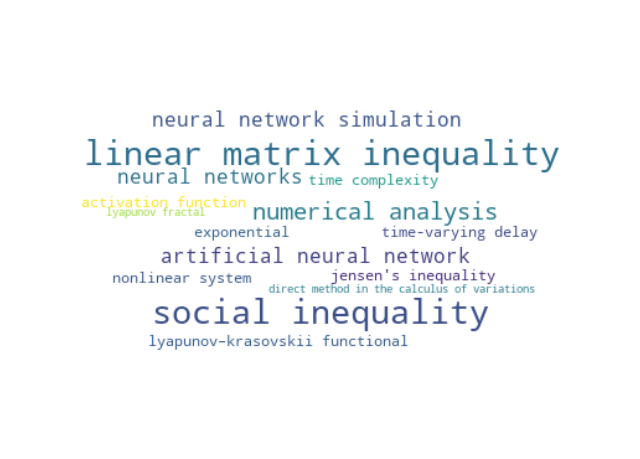
\includegraphics[width=0.495\textwidth]{img/topic1.png}
	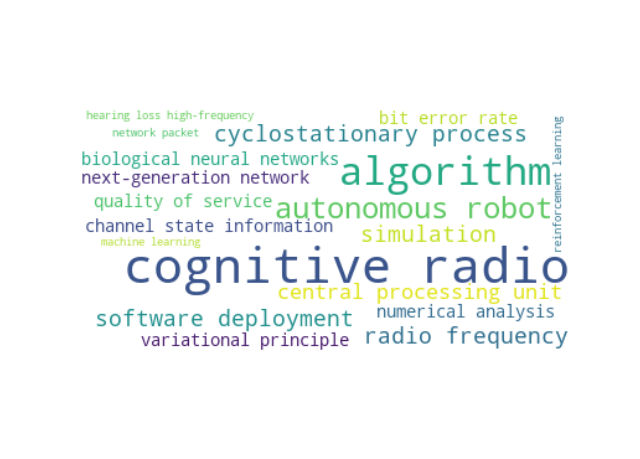
\includegraphics[width=0.495\textwidth]{img/topic2.png}\\
	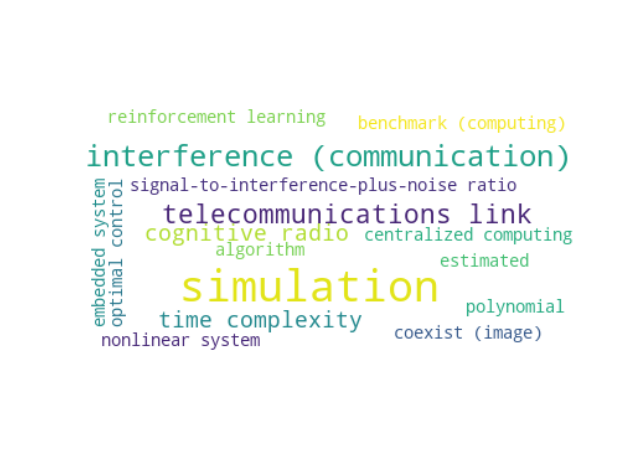
\includegraphics[width=0.495\textwidth]{img/topic3.png}
	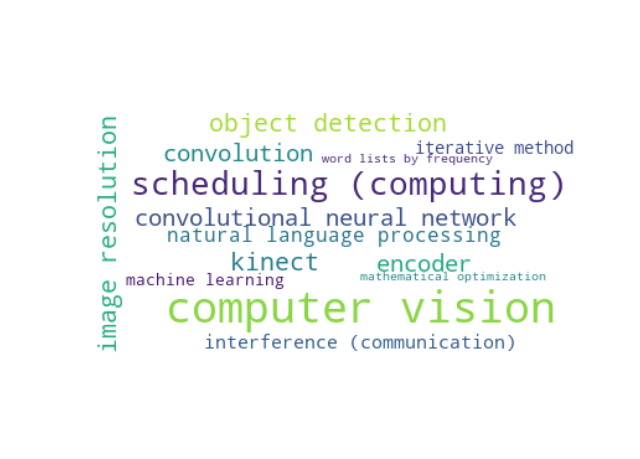
\includegraphics[width=0.495\textwidth]{img/topic4.png}
	\caption{These are some examples of the $K$ time-fused topics, that are computed during \textbf{Task 2}, the frequency of the word in the respective topic-chains is used in order to determine the font-size in the word cloud.}\label{fig:fusedtopics}
\end{figure}

\newpage
\bibliographystyle{unsrt}
\bibliography{ref}